\chapter{Vorgehen}
\label{cha:vorgehen}

%Je nach Art der Arbeit kann diese Kapitelüberschrift auch \glqq Konzeptentwurf\grqq~lauten.
%
%Beschreibung der Ausgangssituation und des Themenumfelds. Ggf. wird darauf eingegangen, welche Randbedingungen und Einflüsse zu beachten sind.
%
%Anforderungsanalyse und Anforderungsdefinition, nach Möglichkeit strukturiert, um zu einem späteren Zeitpunkt die Anforderungen nachvollziehbar verifizieren zu können.
%
%Herleitung einer Lösung (einer Methodik, eines experimentellen Aufbaus oder von unterschiedlichen Konzepten), Lösungsbewertung und bewusste Wahl des gewählten Vorgehens. An dieser Stelle ist auch auf die Zuverlässigkeit einer Methodik oder auf die Genauigkeit von Untersuchungen einzugehen. Die Überlegungen sollen dazu helfen, mit der angestrebten Lösung die gestellten Anforderungen zu erfüllen, um schließlich die Ziele der Arbeit erreichen zu können.
%
%Bei einer Gegenüberstellung von verschiedenen Lösungsansätzen kann z.~B. eine Nutzwertanalyse helfen. Dabei sind nicht nur z.~B. die Funktion, Leistungsfähigkeit, Umsetzbarkeit und Nutzbarkeit, sondern auch z.~B. wirtschaftliche Aspekte, wie Stück-, Entwicklungskosten oder Ressourcenverbrauch zu berücksichtigen. Sehr bedeutend sind auch Aspekte der Nachhaltigkeit unter Betrachtung des gesamten Lebenszyklus einer erarbeiteten Lösung.
%
%Sowohl bei der Anforderungsdefinition, als auch bei der Lösungsfindung gibt es eine große Anzahl an verschiedenen Methoden. Eine kleine Auswahl ist in der folgenden Aufzählung zu finden.
%
%\begin{itemize}
%\item Anforderungsdefinition mithilfe des Requirements Engineering  \autocite{Pohl.2021}
%\item Systems Engineering Ansatz \autocite{Schluter.2023}
%\item Agile Entwicklungsmethodiken \autocite{Cohn.2010, Martin.2020, Wirdemann.2022}
%\item Klassische Bewertungsverfahren \autocite{Breiing.1997, Zangemeister.2014}
%\end{itemize}
%
%Ziel dieses Kapitels ist, dass auf Basis von umfassend und genau formulierten Anforderungen (ggf. auch Nicht-Zielen) eine Lösungsvielfalt erarbeitet wird, welche anschließend strukturiert bewertet wird, um eine fundierte Begründung für die angestrebte Art der Umsetzung herzuleiten.

\section{Anforderung}
\section{Konzept}
\section{Nutzwertanalyse}
\section{Zeitplan}
\begin{figure}[hbt]
\centering
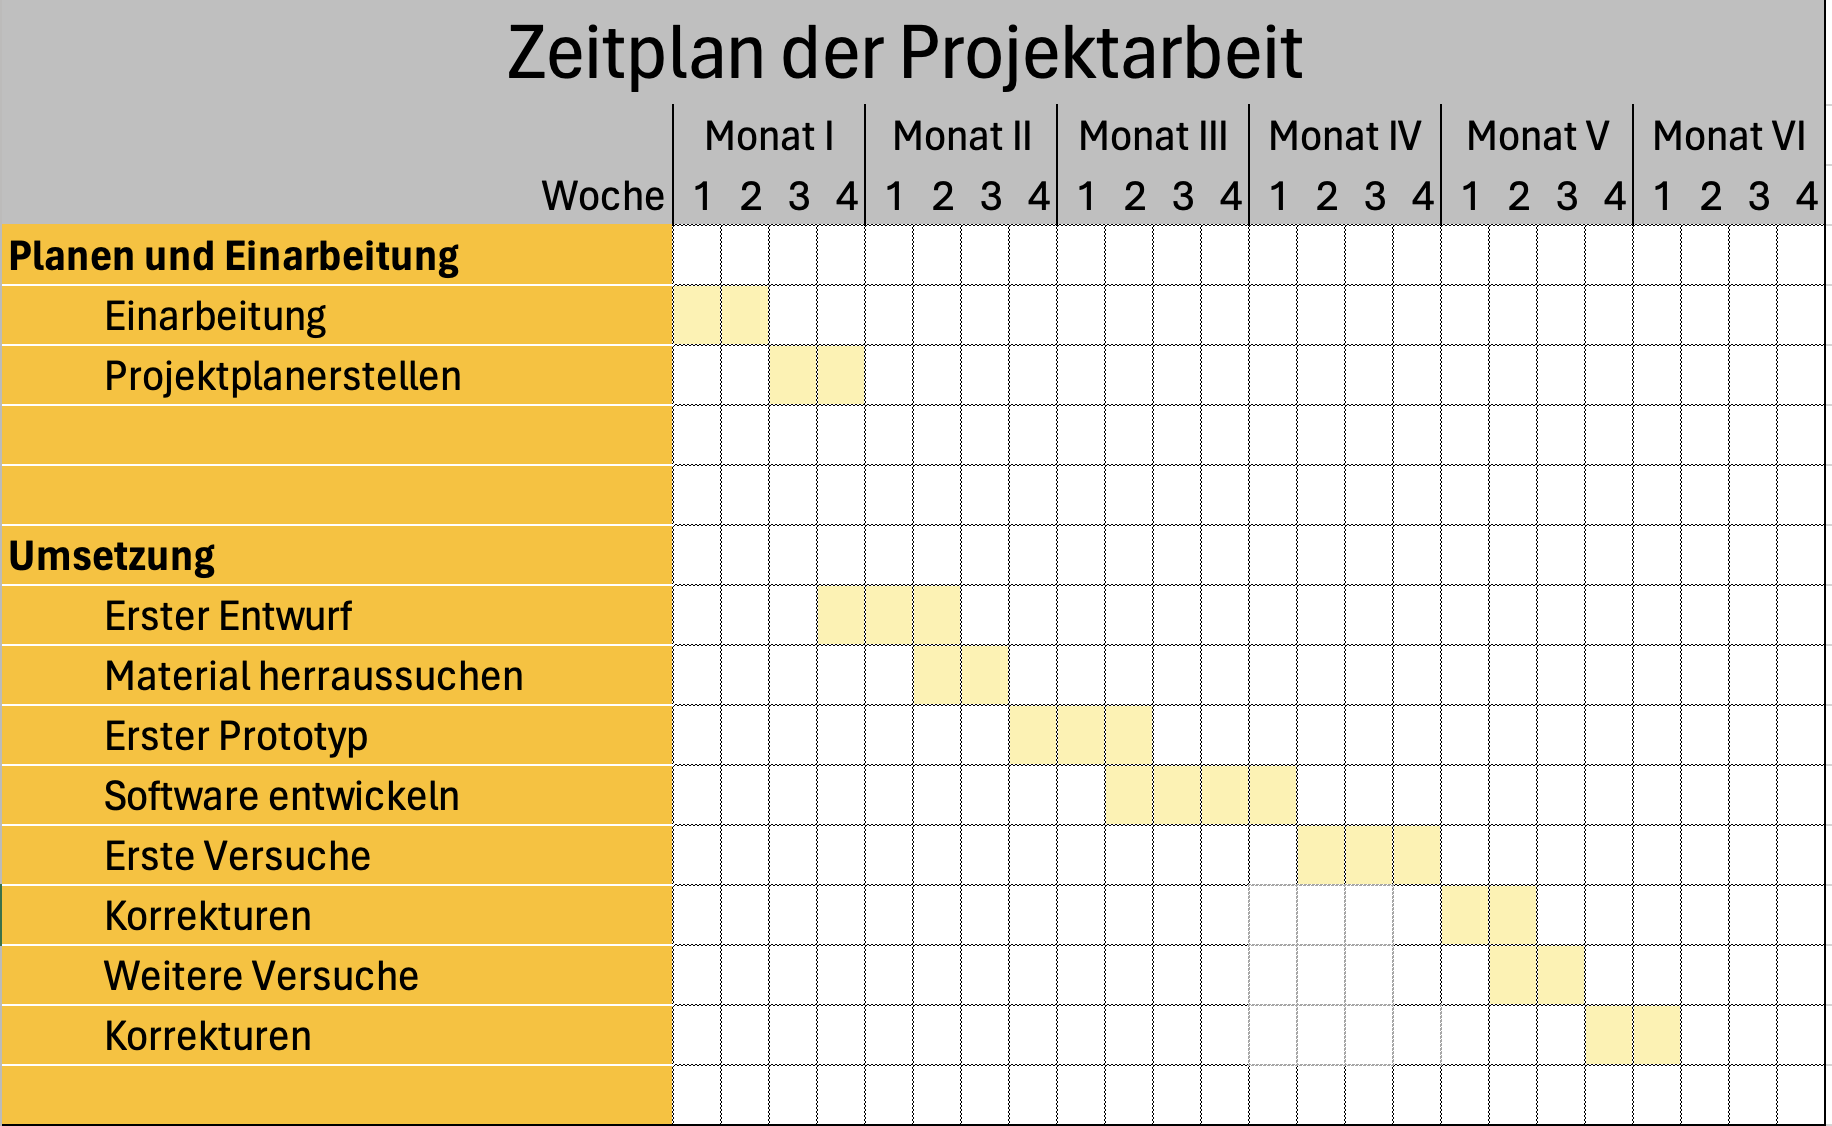
\includegraphics[width=0.9\linewidth]{images/Zeitplan}
\caption[Zeitplan]{ Zeitplan}
\label{fig:Zeitplan}
\end{figure}